\chapter{PROCEDIMENTOS TE\'{O}RICOS E COMPUTACIONAIS}
\label{chap:procedimentos}

Este capítulo descreve detalhadamente os procedimentos teóricos e computacionais adotados para a implementação do Algoritmo de Grover. Inicialmente, apresenta-se o procedimento teórico formalizado matematicamente e expresso por meio de circuitos qu\^{a}nticos compostos por portas lógicas elementares.

Posteriormente, será apresentado o procedimento computacional, que envolve a modelagem e a execução do algoritmo utilizando ferramentas de simulação e programação qu\^{a}ntica. Esta parte tem como objetivo validar teoricamente o funcionamento do algoritmo e analisar, por meio de experimentos práticos, o seu desempenho em ambientes computacionais qu\^{a}nticos. Assim, este capítulo estabelece as bases necessárias para a compreensão e replicação dos resultados obtidos ao longo deste trabalho.

\section{Criando o Circuito Quântico Virtual}
\label{sec: circuitoVirtual}

Nesta seção, serão apresentados de forma integrada os aspectos teóricos e computacionais da implementação do Algoritmo de Grover com $4$ qubits e que orientaram a construção do circuito quântico utilizado no processo. Serão apresentados, também, trechos de código escritos em \emph{Python} utilizando a biblioteca \emph{Qiskit}. A combinação entre fundamentação teórica e simulação computacional permite visualizar com clareza o funcionamento do algoritmo, cujo procedimento foi dividido em três etapas principais:
\begin{enumerate}
    \item a preparação do espaço de pesquisa;
    \item a aplicação do oráculo;
    \item a operação de difusão.
\end{enumerate}

Cada uma dessas etapas é descrita de forma detalhada em uma estrutura que visa garantir clareza na compreensão do funcionamento do circuito e posterior análise dos resultados.

\subsection{Preparação Inicial do Circuito Quântico}
\label{subSec: preparacaoInicialTeo}

A princípio, foi necessário determinar o Espaço de Pesquisa $\ket{s}$, \emph{i. e.}, criar uma superposição uniforme dos estados da base de $4$ qubits. Como sugere a Equação~\ref{eq: superposicao}, para $n=4$ qubits, o Espaço de Pesquisa possui $N = 2^4 = 16$ itens, e é dado por:
%
\begin{align}
    \label{eq: espacoPesquisa}
    \notag
    \ket{s} =&~ \frac{1}{4} \sum_{x=0}^{15} \ket{bin(x)} \\
     =&~ \frac{1}{4} (\ket{0000} +  \ket{0001} +  \ket{0010} +  \ket{0011} +  \ket{0100} +  \ket{0101} +  \ket{0110} + \ket{0111} +  \\
    \notag{}
     &~~~~~\ket{1000} +  \ket{1001} +  \ket{1010} +  \ket{1011} +  \ket{1100} +  \ket{1101} +  \ket{1110} +  \ket{1111})
\end{align}
%
\tab\tab Para a implementação do circuito quântico virtual em \emph{Qiskit}, deve-se primeiramente importar as dependências e instanciar as variáveis do circuito. As dependências relacionadas à biblioteca \emph{Qiskit} são apresentadas na Figura~\ref{cod: dependencias} e a importação e declaração dos recursos na Figura~\ref{cod: inicializacao}.

\begin{figure}[!htb]
\centering
\caption{Dependências do Programa   } 
\begin{minted}{json}
{
  "QiskitDependencies": {
    "qiskit": "2.1.2",
    "qiskit-aer": "0.17.1",
    "qiskit-ibm-provider": "0.11.0",
    "qiskit-ibm-runtime": "0.41.1"
  }
}
\end{minted} 
{\small Fonte: do autor} 
\label{cod: dependencias} 
\end{figure}

\begin{figure}[!htb]
\centering
\caption{Inicialização do Circuito Qu\^{a}ntico} 
\begin{minted}{python}
from qiskit import QuantumCircuit, QuantumRegister, ClassicalRegister

n = <num_qubits>
qubits = QuantumRegister(n, 'qubit')
bits= ClassicalRegister(n, 'bit')

QC_Grover = QuantumCircuit(qubits, bits)
\end{minted} 
{\small Fonte: do autor} 
\label{cod: inicializacao} 
\end{figure}

A Figura~\ref{cod: inicializacao} mostra \verb|QC_Grover|, que é um objeto instanciado pela classe \verb|QuantumCircuit|. Nela será adicionado todo o circuito. Por sua vez, \verb|qubits| e \verb|bits| são instâncias das classes \verb|QuantumRegister| e \verb|ClassicalRegister|, respectivamente, que serão responsáveis pelo armazenamento dos dados e importantes no processo de medição.

A próxima etapa é a formação do espaço de pesquisa mencionado anteriormente e, para isso, pode-se recorrer à Equação~\ref{eq: preparacaoInicial}, que implica no uso de portas $Hadamard$ em cada \emph{qubit}. Esse passo é feito usando o módulo \verb|inicializa_s|, apresentado na Figura~\ref{cod: preparacao}.

\begin{figure}[!htb]
\centering
\caption{Módulo Preparação Inicial} 
\begin{minted}{python}
def inicializa_s(qc, qubits):
    for qubit in qubits:
        qc.h(qubit)
    return qc
\end{minted} 
{\small Fonte: do autor} 
\label{cod: preparacao} 
\end{figure}

Uma representação visual do circuito quântico virtual relativo a este trecho pode ser acompanhada na Figura~\ref{fig: preparacaoInicial}. É relevante notar que todos os \textit{qubits} são inicializados no estado $\ket{0}$.
%
\begin{figure}[!htb]
    \centering
    \caption{Circuito Quântico Virtual - Superposição}
    \label{fig: preparacaoInicial} 
    
    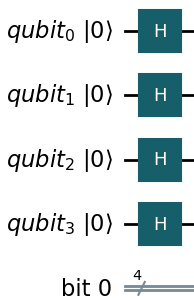
\includegraphics[scale=0.5]{Imagens/preparacaoInicial.png}

    \vspace{0.3em}
    {\small Fonte: do autor} % Fonte da imagem
\end{figure}
%
\subsection{Or\'{a}culo}
\label{subSec: oraculoTeo}

Para dar prosseguimento, é preciso marcar o estado que se deseja obter, \emph{i. e.}, aplicar o \nameref{subSec: oraculoAlg} (Equaç\~{a}o~\ref{eq: fx Oraculo}) ao Espaço de Pesquisa (Equaç\~{a}o~\ref{eq: espacoPesquisa}). Seja $\omega = \ket{1111}$ o estado arbitrariamente escolhido para ser buscado, a aplicação do Oráculo é tal que
%
\begin{align}
    \notag
    U_f\ket{s} = ~& \frac{1}{4}~U_f~[\ket{0000} + \ket{0001} + \ket{0010} + \ket{0011} + \ket{0100} + \ket{0101} + \ket{0110} +\ket{0111} + \\ \notag
    &~ \ket{1000} + \ket{1001} + \ket{1010} + \ket{1011} + \ket{1100} + \ket{1101} + \ket{1110} + \ket{1111}] \\
    \label{eq: aplicacaoOraculo}
    = &~ \frac{1}{4}(\ket{0000} + \ket{0001} + \ket{0010} + \ket{0011} + \ket{0100} + \ket{0101} + \ket{0110} +\ket{0111} + \\ \notag
    &~ \ket{1000} + \ket{1001} + \ket{1010} + \ket{1011} + \ket{1100} + \ket{1101} + \ket{1110} + -\ket{1111})
\end{align}
%
Que pode ser expresso de acordo com a matriz $16 \times 16$
%
\begin{equation*}
    (U_{f}~\ket{s})_{[16 \times 16]} = \begin{bmatrix}
        1 & 0 &  \cdots  & 0\\
        0 & 1 &  \cdots  & 0\\
        \vdots & \vdots & \ddots & \vdots \\
        0 & 0 &  \cdots  & -1\\
    \end{bmatrix}_{[16 \times 16]} 
    \label{mtx: aplicacaoOraculo}
\end{equation*}

O desafio seguinte foi determinar a(s) porta(s) lógica(s) que retorna(m) essa matriz. Para isso, pode-se seguir a regra de formação enunciada na Seção~\ref{subSec: oraculoAlg} do Capítulo~\nameref{chap: ferramentas}. Como o estado buscado é $\omega = \ket{1111}$, não será necessário o uso de portas $X$, apenas uma $MCZ$ (Equação~\ref{mtx: gateMCZ}) será suficiente, pois o resultado prático que se obtém com a aplicação da porta $MCZ$ é basicamente mudar a fase do último elemento da matriz $N \times N$ à qual ela for aplicada, exatamente o que se intenta obter; portanto, o Oráculo será uma porta $MCZ$.

Em \emph{Qiskit}, a implementação é feita com o módulo \verb|oraculo_Uw|, mostrado na Figura~\ref{cod: oraculo}. E o circuito quântico virtual relativo a este trecho é mostrado na Figura~\ref{fig: aplicacaoOraculo}\footnote
{
Como o \emph{Qiskit} não oferece suporte nativo à porta $MCZ$, ela é construída combinando portas $Hadamard$ e $MCX$, visto que $MCZ=H~MCX~H$ ($H$'s apenas no qubit alvo).

[TALVEZ DEMONSTRAR NO APÊNDICE***]
}.

\begin{figure}[!thb]
\centering
\caption{Módulo Oráculo} 
\begin{minted}{python}
def mcz_circ(qc):
    qc.h(3)
    qc.mcx([0, 1, 2], 3)
    qc.h(3)
    return qc
    
def oraculo_Uw(qc, qubits, winner, QuantumCircuit):
    for i, index in enumerate(winner):
        if index == "0":
            qc.x(i)

    # Para agrupar as portas H MCX H em uma MCZ
    mcz_gate = mcz_circ(qc = QuantumCircuit(4,name="mcz")).to_instruction() 
    qc.append(mcz_gate,[i for i in range(4)])

    for i, index in enumerate(winner):
        if index == "0":
            qc.x(i)
\end{minted} 
{\small Fonte: do autor} 
\label{cod: oraculo} 
\end{figure}

O módulo \verb|mcz_circ| apenas é usado para agrupar o conjunto de portas $H~MCX~H$ em um único bloco, para facilitar identificação. Para fins de ilustração, vide Figura~\ref{fig: aplicacaoOraculo}. O parâmetro \texttt{winner} representa o estado marcado a ser identificado (por exemplo, $\ket{1111}$).

\begin{figure}[!htb]
    \centering
    \captionsetup{justification=centering}
    \caption{Circuito Quântico Virtual - Oráculo}
    \label{fig: aplicacaoOraculo}

    \begin{subfigure}[b]{0.16\textwidth}
        \centering
        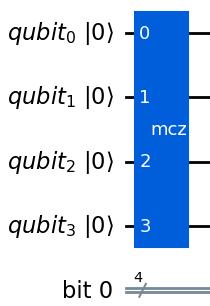
\includegraphics[width=\textwidth]{Imagens/oraculoContraido.png}
        \caption{Oráculo contraído.}
        \label{subfig: oraculoContraido}
    \end{subfigure}
    \hspace{1cm}
    \begin{subfigure}[b]{0.25\textwidth}
        \centering
        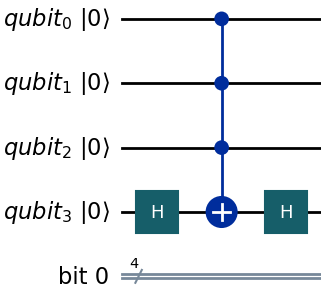
\includegraphics[width=\textwidth]{Imagens/oraculoExpandido.png}
        \caption{Oráculo expandido.}
        \label{subfig: oraculoExpandido}
    \end{subfigure}

    \vspace{0.3em}
    {\small Fonte: do autor.}
\end{figure}
%
\subsection{Difus\~{a}o}
\label{subSec: difusaoTeo}

A etapa seguinte é a de amplificação do estado buscado, aplicando uma segunda reflexão $U_s$ (Equaç\~{a}o~\ref{eq:Us}) na resultante da etapa anterior. Conforme demonstrado na Seção~\ref{subsec:difusaoAlg}, Capítulo~\nameref{chap: ferramentas}, a operação que se deseja realizar é dada pela Equação~\ref{eq:aplicacaoDifusao}. Essa operação aplica uma fase negativa a todos os estados ortonormais a $\ket{0}$, \emph{i. e.}, a expansão da Equação~\ref{eq:aplicacaoDifusao} para quatro qubits resulta em:

\begin{equation}
U_0~\ket{s} = \ket{0000} - \ket{0001} - \ket{0010} - \ket{0011} - \cdots - \ket{1111} 
\end{equation}

Ou seja, a amplitude $\ket{0000}$ aumenta em relação aos demais que invertem.

O difusor é representado pela matriz:

\begin{equation}
U_0 = -
\begin{pmatrix}
-1 & 0 & \cdots & 0 \\
0 & 1 & \cdots & 0 \\
\vdots & \vdots & \ddots & \vdots \\
0 & 0 & \cdots & 1
\end{pmatrix}
\label{mtx: Difusao}
\end{equation}

Para colocar isso em termos de portas lógicas, basta utilizar o conjunto de portas apresentado pela Equação~\ref{gate: operadorDifusaoCompleto}. Em \emph{Qiskit}, a implementação pode ser feita com o uso do módulo \verb|difusor_Us|, visto na Figura~\ref{cod: difusao}.

\begin{figure}[!hb]
\centering
\caption{Módulo Operador de Difusão} 
\begin{minted}{python}
def difusor_Us(qc, qubits):
    for i in qubits:
        qc.h(i)
        qc.x(i)

    # Para agrupar as portas H MCX H em uma MCZ
    mcz_gate = mcz_circ(qc = QuantumCircuit(4,name="mcz")).to_instruction() 
    qc.append(mcz_gate,[i for i in range(4)])

    for i in qubits:
        qc.x(i)
        qc.h(i)
    return qc
\end{minted} 
{\small Fonte: do autor} 
\label{cod: difusao} 
\end{figure}

A idealização virtual desse trecho pode ser observada na Figura~\ref{fig: difusaoCompleto}. Nela, é possível fazer a equivalência entre $U_0$ (Equação~\ref{gate: difusor}) e a Figura~\ref{subFig: Uo} e entre $U_s$ (Equação~\ref{gate: operadorDifusaoCompleto}) e a Figura~\ref{subFig: Us}.
%
\begin{figure}[ht!]
    \centering
    \captionsetup{justification=centering}
    \caption{Circuito Qu\^{a}ntico Virtual - Amplificação, $U_0$ e $U_s$.}
    \label{fig: difusaoCompleto}

    \begin{subfigure}[b]{0.25\textwidth}
        \centering
        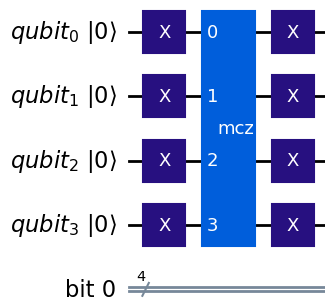
\includegraphics[width=\linewidth]{Imagens/circuitoDifusor.png}
        \caption{Circuito de $U_0$}
        \label{subFig: Uo}
    \end{subfigure}
    \hspace{1cm}
    \begin{subfigure}[b]{0.35\textwidth}
        \centering
        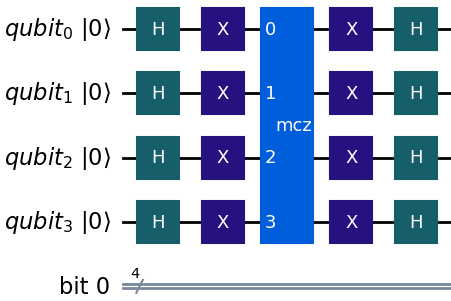
\includegraphics[width=\linewidth]{Imagens/circuitoDifusorCompleto.png}
        \caption{Circuito de $U_s$}
        \label{subFig: Us}
    \end{subfigure}
    
    \vspace{0.3em}
    {\small Fonte: do autor} 
\end{figure}

\subsection{Fator \emph{k}}

Para que a Equação~\ref{eq:psi k} seja de fato satisfeita, deve-se determinar o fator de otimização, \emph{i. e.}, a quantidade de vezes que o \nameref{subsec:oraculoAlg} e o \nameref{subsec:difusaoAlg} devem ser repetidos. O valor de $k$ pode ser obtido com a utilização da Equação~\ref{eq:k value}, em que tem-se $N=16$ e $m=1$.
%
\begin{align*}
    k =&~ \frac{\pi}{4}\sqrt{\frac{N}{m}}\\
    =&~ \frac{\pi}{4}\sqrt{16}\\
    =&~ \pi
\end{align*}
E como $k$ não pode ser número de ponto flutuante, deve-se arredondar para o inteiro mais próximo, ou seja, para fins práticos,
\begin{equation}
    k = 3
    \label{eq: k = 3}
\end{equation}.
Nesse ponto, tem-se que todas as etapas estão concluídas, cabendo, então, uní-las em um único circuito qu\^{a}ntico. Em \emph{Qiskit}, isso pode ser feito com o trecho de código mostrado na Figura~\ref{cod: geraCircuitoCompleto}, que leva em consideração o valor de $k$, por meio de um \textit{loop} \verb|for| no intervalo dado por $k$. Ao final, aplica-se o método \verb|measure()| ao circuito, que realiza a medição dos \textit{qubits}, colapsando o sistema em um dos estados da base computacional, revelando o resultado da busca.

\begin{figure}[!htb]
\centering
\caption{Trecho para formação do Circuito Quântico Virtual.} 
\begin{minted}{python}
N = 2**n
k = (round((pi/4)*sqrt(N)))
marked_state = "<seu_estado>"
inicializa_s(QC_Grover, range(n))

for _ in range(k):
    QC_Grover.barrier([i for i in range(n)])
    oraculo_Uw(QC_Grover, range(n), marked_state, QuantumCircuit)
    difusor_Us(QC_Grover, (range(n)))

QC_Grover.barrier([i for i in range(n)])
QC_Grover.measure([0,1,2,3],[0,1,2,3])
\end{minted} 
{\small Fonte: do autor} 
\label{cod: geraCircuitoCompleto} 
\end{figure}

O circuito relativo ao trecho em questão pode ser visto na Figura~\ref{fig: circuitoCompleto}. As barreiras (\texttt{barrier()}), nesse caso, são apenas separadores visuais do processo de iteração, e os objetos ao final de cada canal indicam o processo de medição do estado final sendo armazenado nos canais clássicos.

\begin{figure}[!thb]
    \centering
    \captionsetup{justification=centering}
    \caption{Circuito Quântico Virtual - Algoritmo de Grover Completo.}
    \label{fig: circuitoCompleto}
    
    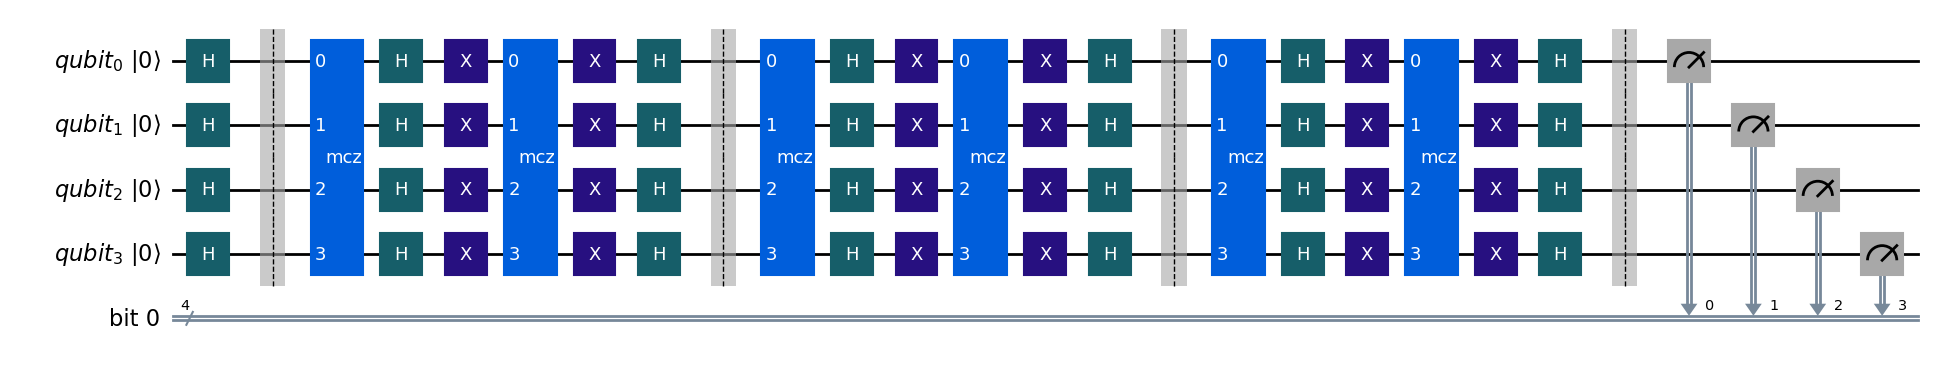
\includegraphics[width=\linewidth]{Imagens/circuitoCompleto.png}

    \vspace{0.1em}
    {\small Fonte: do autor} 
\end{figure}
\section{Plataforma \textit{IBM Quantum}}
\label{sec: plataformaIBM}

Nesta seção, descreve-se e elucida-se por meio de trechos de códigos exemplos o procedimento adotado para o acesso e preparação da simulação do circuito do Algoritmo de Grover utilizando os recursos computacionais da \textit{IBM Quantum Platform} \cite{IBM_quantum}. Essa plataforma online desenvolvida pela IBM permite a execução de algoritmos em computadores quânticos reais e simuladores avançados disponíveis na nuvem.

O primeiro passo consiste na criação de uma conta na plataforma e posterior autenticação com uma organização habilitada. Dentro do ambiente web, o usuário pode configurar projetos e acessar diferentes dispositivos quânticos, incluindo simuladores ideais (sem ruído), simuladores com ruído e \textit{hardwares} reais. Cada projeto está vinculado a uma \textit{instância}, que define os recursos disponíveis, como prioridade de fila e acesso a dispositivos específicos.

Diferentemente dos ambientes locais de simulação, como os disponíveis via \texttt{AerSimulator} no \textit{Qiskit}, a \textit{IBM Quantum} exige que até mesmo as simulações ideais sejam submetidas remotamente, exigindo autenticação prévia e conexão à nuvem. Com a migração da plataforma para o novo modelo unificado, o canal de acesso deve ser definido como \verb|ibm_quantum_platform|, e é obrigatória a definição explícita da \textit{instância}.

\subsection{Procedimento de Autenticação}
\label{subSec: auth}

A seguir, a Figura~\ref{cod: acessaIBM} apresenta um exemplo do código utilizado para salvar e autenticar uma conta na plataforma, utilizando a biblioteca \verb|qiskit_ibm_runtime|:

\begin{figure}[!htb]
\centering
\caption{Trecho de acesso à \textit{IBM Quantum Platform}.} 
\begin{minted}{python}
from qiskit_ibm_runtime import QiskitRuntimeService

QiskitRuntimeService.save_account(
    token="<seu_token>",
    instance="<sua_instancia>",
    channel="ibm_quantum_platform",
    overwrite=True,
    set_as_default=True
)
service = QiskitRuntimeService()
\end{minted} 
{\small Fonte: do autor} 
\label{cod: acessaIBM} 
\end{figure}

O \texttt{token} pode ser obtido no perfil do usuário na plataforma, enquanto a \texttt{instance} segue o padrão \texttt{<hub>/<group>/<project>}, que pode ser consultado no painel de gerenciamento de projetos da \textit{IBM Quantum Platform}. A chamada \verb|set_as_default=True| permite que o serviço seja usado diretamente nos próximos acessos, sem necessidade de repetir a autenticação.

Após essa configuração inicial, torna-se possível listar os dispositivos disponíveis, verificar seus estados (como filas, fidelidades e número de qubits), selecionar o \textit{backend} desejado e submeter os circuitos para execução.

\subsection*{Fluxo de Execução na Nuvem}

O processo completo de execução de um circuito na plataforma envolve:

\begin{itemize}
    \item Construção do circuito com bibliotecas do \texttt{Qiskit};
    \item Escolha do \textit{backend} apropriado (simulador ou QPU);
    \item Submissão da tarefa à nuvem via \texttt{QiskitRuntimeService};
    \item Acompanhamento da execução e análise dos resultados.
\end{itemize}

\subsection{Simulação Ideal via \texttt{Statevector}}
\label{subSec: simulacaoIdeal}

Essa seção traz um exemplo de código que gera uma distribuição de probabilidades ideal, utilizando a classe \texttt{Statevector} do \texttt{Qiskit}, apresentada na Figura~\ref{cod: simulacaoIdeol}, que simula a evolução do estado quântico de forma exata e livre de ruído. Essa abordagem fornece a expectativa teórica para o comportamento do algoritmo de Grover.

\begin{figure}[!htb]
\centering
\caption{Trecho para Simulação Ideal.} 
\begin{minted}{python}
from qiskit.quantum_info import Statevector
ideal_distribution = Statevector.
                     from_instruction(QC_Grover).
                     probabilities_dict()
fig, ax = plt.subplots()
plot_histogram(ideal_distribution, 
               title="Distribuição Ideal de Probabilidades",
               ax=ax)
ax.set_ylabel("Probabilidade")
plt.show()
\end{minted}
{\small Fonte: do autor} 
\label{cod: simulacaoIdeol} 
\end{figure}

Este resultado serve como referência teórica da máxima fidelidade, permitindo a comparação com as demais execuções e a análise da influência dos ruídos nos sistemas quânticos reais.

\subsection{Simulação com Ruído via \textit{AerSimulator}}
\label{subSec: simulacaoRuido}

Essa seção apresenta uma simulação mais próxima da realidade, pois faz uso de informações de ruído da QPU escolhida (definindo \texttt{<nome\_backend>}). Para isso, utiliza a classe \texttt{AerSimulator}, da biblioteca \texttt{qiskit\_aer}. O código exemplo é mostrado na Figura~\ref{cod: simulacaoRuido}. Essa é uma forma de criar uma simulação que busca imitar de forma mais precisa o comportamento prático do circuito, uma vez que a simulação com ruído permite observar a degradação de fidelidade causada por imperfeições reais nos dispositivos quânticos.

\begin{figure}[!htb]
\centering
\caption{Trecho para Simulação com Ruído.} 
\begin{minted}{python}
from qiskit_aer import AerSimulator
from qiskit.compiler import transpile

service = QiskitRuntimeService()
backend = service.backend('<nome_backend>')

# Gerar simulador com modelo de ruído real
backend_sim = AerSimulator.from_backend(backend)
transpiled_circ_sim = transpile(QC_Grover, backend_sim)
result = backend_sim.run(transpiled_circ_sim, shots=<num_shots>).result()
circuits.append(transpiled_circ_sim)
\end{minted}
{\small Fonte: do autor} 
\label{cod: simulacaoRuido} 
\end{figure}

Essa abordagem é valiosa para testar e validar circuitos antes da submissão ao \textit{hardware} físico, permitindo ajustes e observação de efeitos de ruído específicos, como erros de porta, leitura e decoerência.

\subsection{Execução em  via \texttt{Sampler}}
\label{subSec: execucaoQPU}

Por fim, essa última seção traz os procedimentos a serem realizados para a execução em uma QPU. Antes de o circuito ser enviado a alguma QPU propriamente dita, ele precisa ser reescrito em uma linguagem que ela entenda, \textit{i. e.}, o circuito virtual precisa ser reescrito em termos das portas base do \textit{backend} no qual se pretende enviá-lo. Essa é a etapa de compilação mencionada na Seção~\ref{subSec: computadores} e sua implementação é feita com a função \texttt{transpile} conforme mostrado na Figura~\ref{cod: compilacao}.

\begin{figure}[!htb]
\centering
\caption{Trecho para Compilação.} 
\begin{minted}{python}
from qiskit.compiler import transpile

backend_HW = service.backend("<nome_backend>")
transpiled = transpile(QC_Grover, backend_HW, optimization_level=<optim_lvl>)
\end{minted}
{\small Fonte: do autor} 
\label{cod: compilacao} 
\end{figure}

A definição de <\texttt{nome\_backend}> é o que garante a compilação ideal de acordo com as portas base de cada \textit{backend}, visto que cada tipo de processador pode possuir portas base diferentes. Pode-se também configurar o nível de otimização, explanado na Seção~\ref{subSubSec: otimizacao}, por meio de \texttt{optimization\_level}. Concluída essa etapa, segue-se com o circuito compilado.

A Figura~\ref{cod: execucaoSampler} mostra um trecho de exemplo para execução em QPU's que possibilita também utilizar as técnicas de supressão -- \textit{Dynamical Decoupling} (DD) e \textit{Pauli Twirling} introduzidas na Seção~\ref{subSec: supressao} -- disponíveis na classe \texttt{Sampler} da biblioteca \texttt{qiskit\_ibm\_runtime}.

\begin{figure}[!htb]
\centering
\caption{Trecho para Execução em QPU via \texttt{Sampler}.} 
\begin{minted}{python}
from qiskit_ibm_runtime import SamplerV2 as Sampler, Batch

def rodar():
    num_shots = <num_shots>
    with Batch(backend=backend_HW):
        sampler = Sampler()
        # Execução com Dynamical Decoupling + Pauli Twirling
        sampler.options.dynamical_decoupling.enable = True
        sampler.options.twirling.enable_gates = True
        job_DD_Twiling = sampler.run([transpiled], shots=num_shots)
try:
    rodar()
except Exception as e:
    print(f"Erro: {e}")
\end{minted}
{\small Fonte: do autor} 
\label{cod: execucaoSampler} 
\end{figure}

A Figura~\ref{cod: execucaoEstimate}, por sua vez, mostra um trecho de exemplo para execução em QPU's que possibilita utilizar as técnicas de mitigação -- \textit{Twirled Readout Error eXtinction} (TREX), \textit{Zero-Noise Extrapolation} (ZNE), \textit{Probabilistic Error Amplification} (PEA), e \textit{Probabilistic Error Cancellation} (PEA) introduzidas na Seção~\ref{subSec: mitigacao} -- disponíveis na classe \texttt{Estimate} da biblioteca \texttt{qiskit\_ibm\_runtime}.

\begin{figure}[!htb]
\centering
\caption{Trecho para Execução em QPU via \texttt{Estimate}.} 
\begin{minted}{python}

COLOCAR CODIGO COM ESTIMATE***

\end{minted}
{\small Fonte: do autor} 
\label{cod: execucaoEstimate} 
\end{figure}

A execução real permite não apenas verificar a eficiência do algoritmo em ambiente prático, mas também comparar os efeitos das técnicas de supressão aplicadas, ajudando a entender o comportamento dos sistemas quânticos sob influência de ruído quântico.



\input{Secoes/ExecucaoQC}

